\documentclass{article}
\usepackage[utf8]{inputenc}
\usepackage[margin=1in]{geometry}
\usepackage{float}
\usepackage{tikz}
\usepackage{tikz-qtree}

\title{Data Structures: Problem Set 5}
\author{Jackie Luo}
\date{April 29, 2015}

\begin{document}
\maketitle

\section{Theory}

\subsection{}
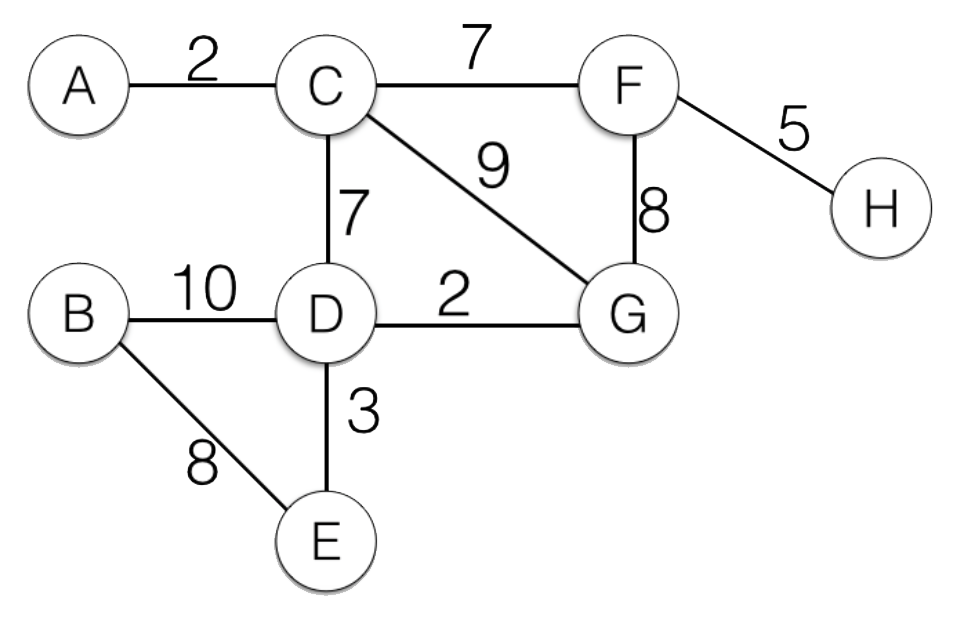
\includegraphics[scale=0.25]{graph.png}
\newline
(A, C) = 2
\newline
(D, G) = 2
\newline
(D, E) = 3
\newline
(F, H) = 5
\newline
(C, D) = 7
\newline
(C, F) = 7
\newline
(B, E) = 8
\newline
(F, G) = 8
\newline
(C, G) = 9
\newline
(B, D) = 10
\newline

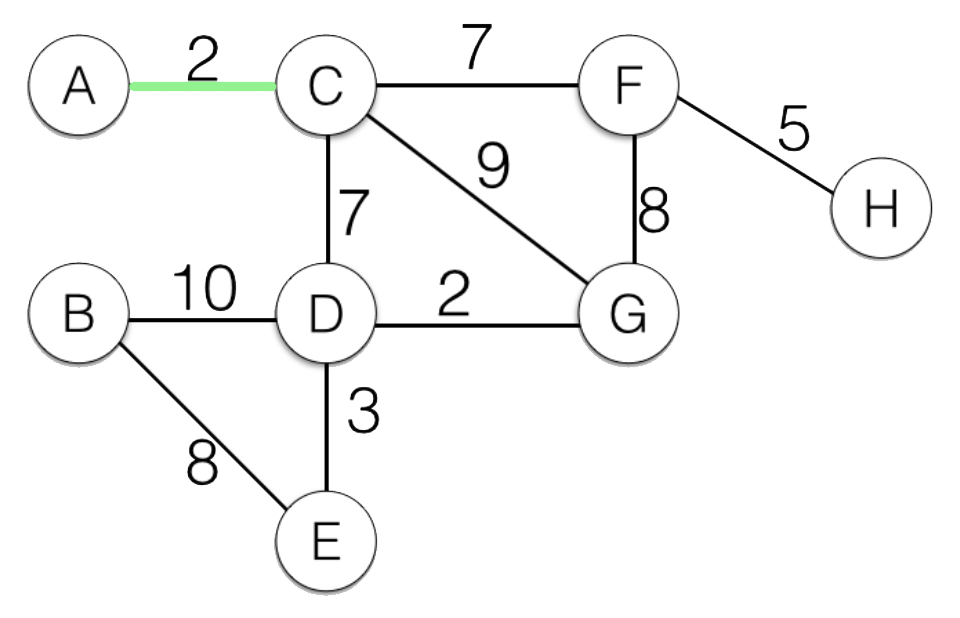
\includegraphics[scale=0.25]{graph1.png}
\newline
(A, C) = 2, OKAY
\newline
(D, G) = 2
\newline
(D, E) = 3
\newline
(F, H) = 5
\newline
(C, D) = 7
\newline
(C, F) = 7
\newline
(B, E) = 8
\newline
(F, G) = 8
\newline
(C, G) = 9
\newline
(B, D) = 10

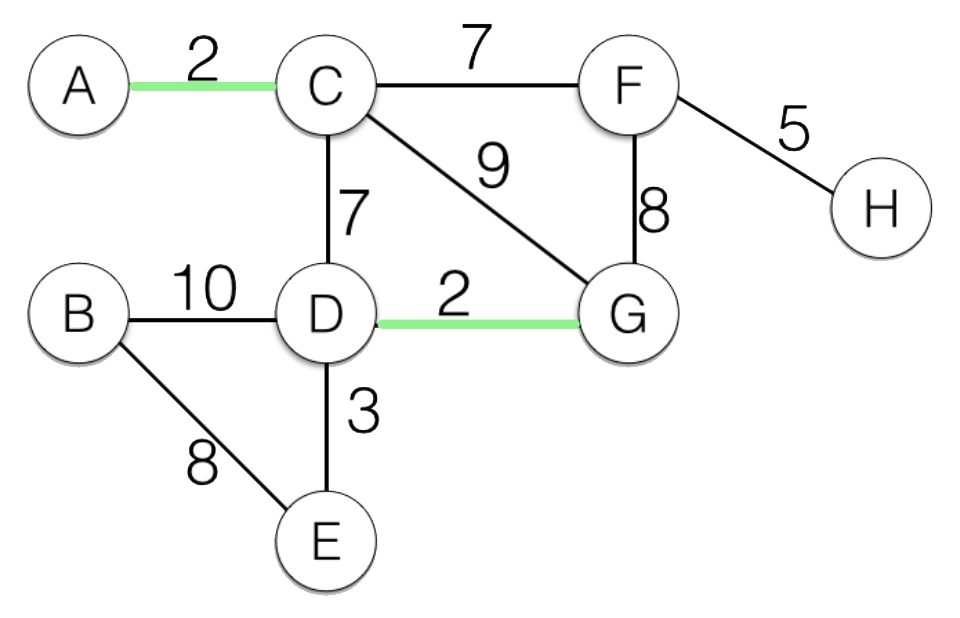
\includegraphics[scale=0.25]{graph2.png}
\newline
(A, C) = 2, OKAY
\newline
(D, G) = 2, OKAY
\newline
(D, E) = 3
\newline
(F, H) = 5
\newline
(C, D) = 7
\newline
(C, F) = 7
\newline
(B, E) = 8
\newline
(F, G) = 8
\newline
(C, G) = 9
\newline
(B, D) = 10

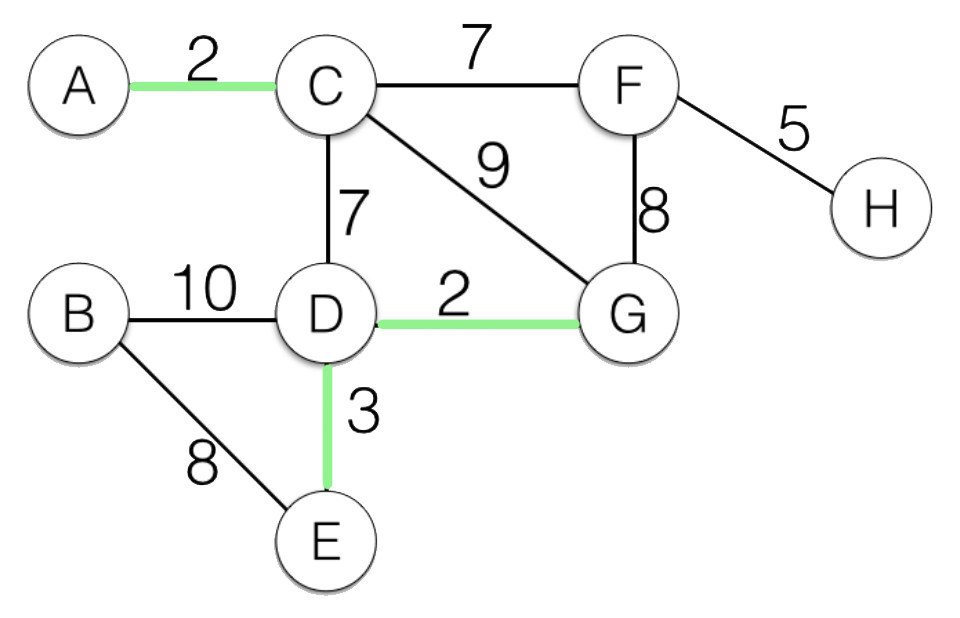
\includegraphics[scale=0.25]{graph3.png}
\newline
(A, C) = 2, OKAY
\newline
(D, G) = 2, OKAY
\newline
(D, E) = 3, OKAY
\newline
(F, H) = 5
\newline
(C, D) = 7
\newline
(C, F) = 7
\newline
(B, E) = 8
\newline
(F, G) = 8
\newline
(C, G) = 9
\newline
(B, D) = 10

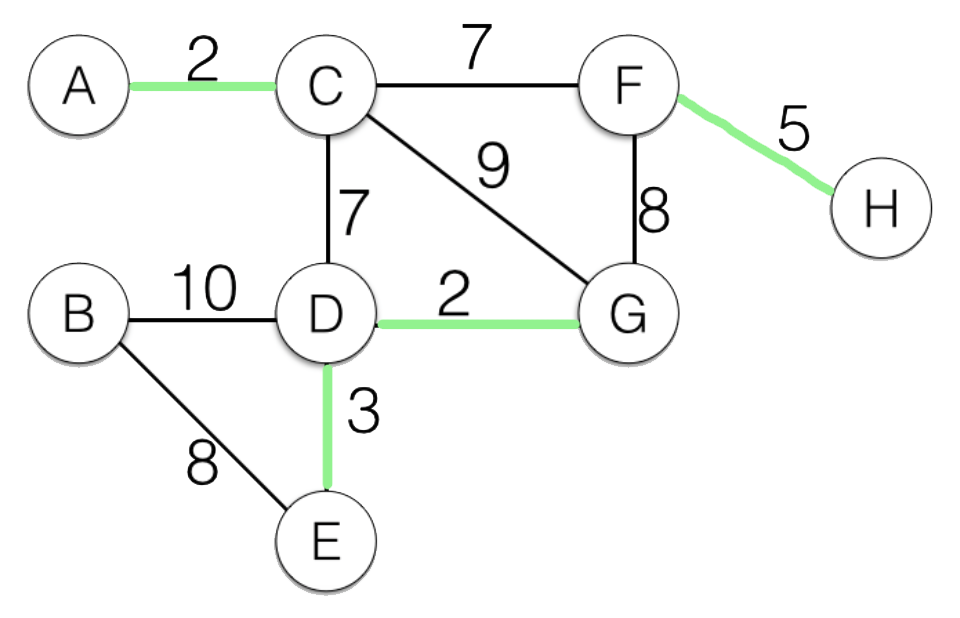
\includegraphics[scale=0.25]{graph4.png}
\newline
(A, C) = 2, OKAY
\newline
(D, G) = 2, OKAY
\newline
(D, E) = 3, OKAY
\newline
(F, H) = 5, OKAY
\newline
(C, D) = 7
\newline
(C, F) = 7
\newline
(B, E) = 8
\newline
(F, G) = 8
\newline
(C, G) = 9
\newline
(B, D) = 10

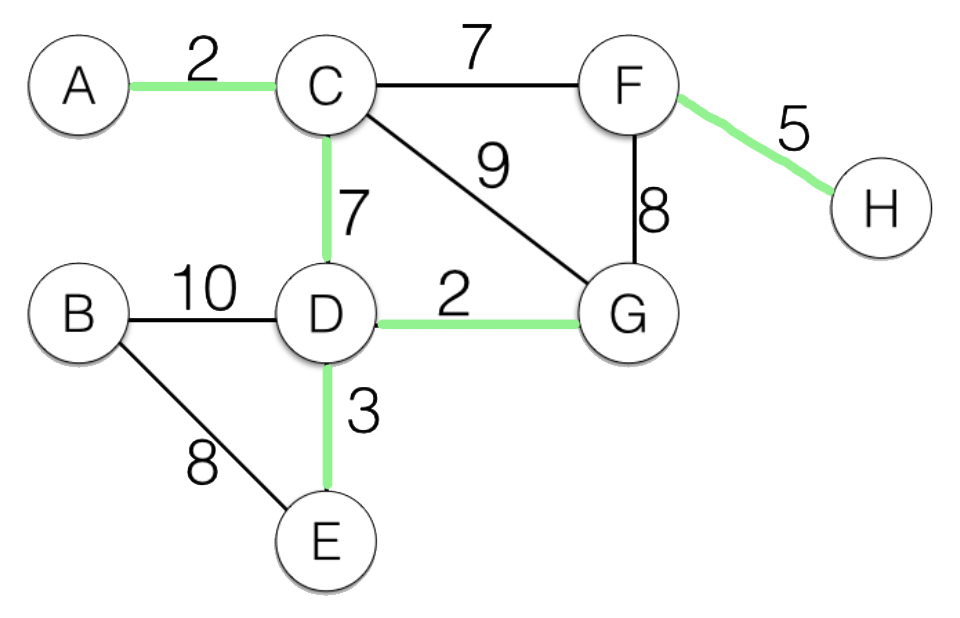
\includegraphics[scale=0.25]{graph5.png}
\newline
(A, C) = 2, OKAY
\newline
(D, G) = 2, OKAY
\newline
(D, E) = 3, OKAY
\newline
(F, H) = 5, OKAY
\newline
(C, D) = 7, OKAY
\newline
(C, F) = 7
\newline
(B, E) = 8
\newline
(F, G) = 8
\newline
(C, G) = 9
\newline
(B, D) = 10

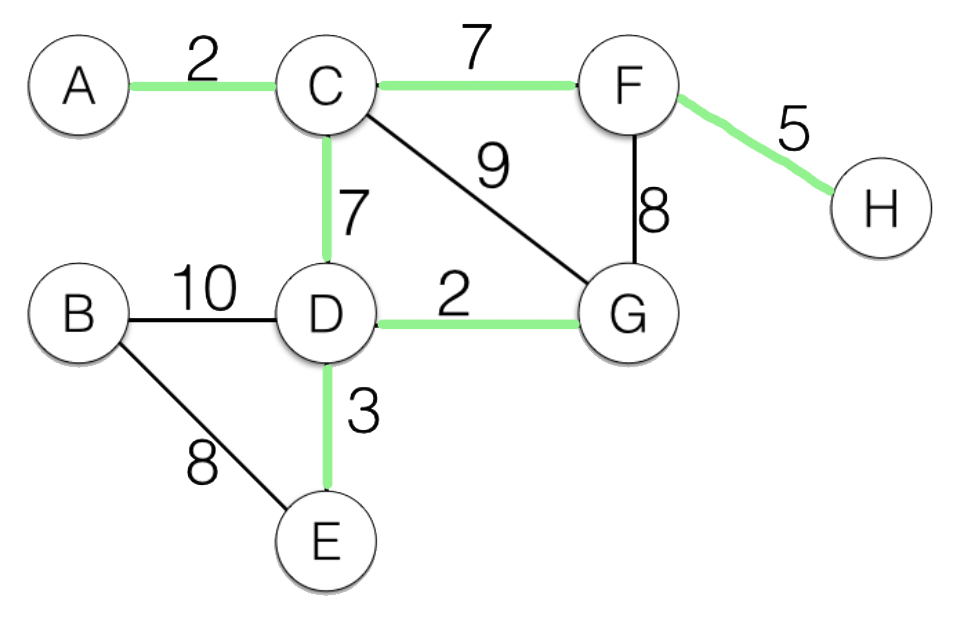
\includegraphics[scale=0.25]{graph6.png}
\newline
(A, C) = 2, OKAY
\newline
(D, G) = 2, OKAY
\newline
(D, E) = 3, OKAY
\newline
(F, H) = 5, OKAY
\newline
(C, D) = 7, OKAY
\newline
(C, F) = 7, OKAY
\newline
(B, E) = 8
\newline
(F, G) = 8
\newline
(C, G) = 9
\newline
(B, D) = 10

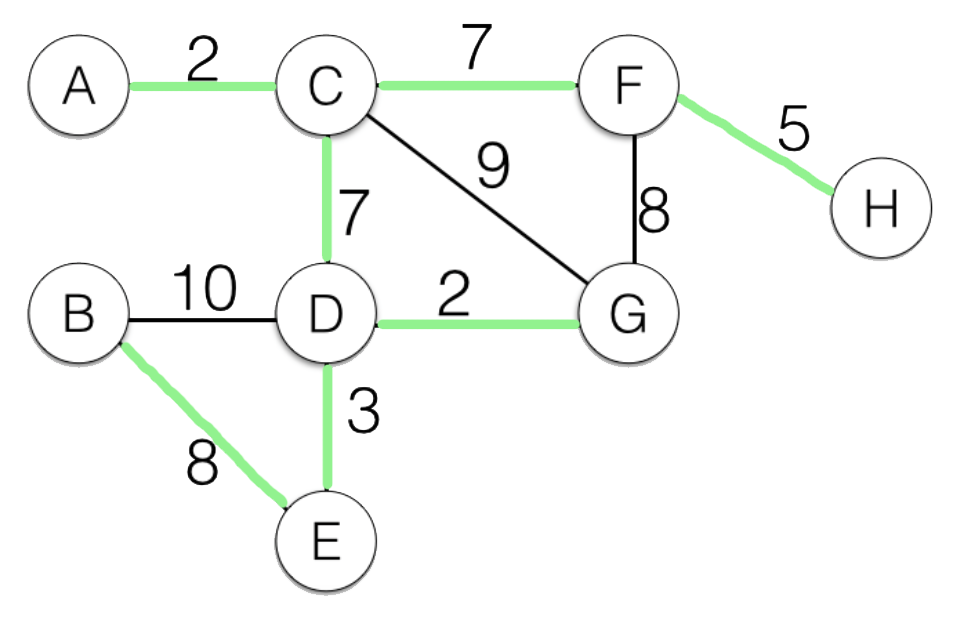
\includegraphics[scale=0.25]{graph7.png}
\newline
(A, C) = 2, OKAY
\newline
(D, G) = 2, OKAY
\newline
(D, E) = 3, OKAY
\newline
(F, H) = 5, OKAY
\newline
(C, D) = 7, OKAY
\newline
(C, F) = 7, OKAY
\newline
(B, E) = 8, OKAY
\newline
(F, G) = 8
\newline
(C, G) = 9
\newline
(B, D) = 10

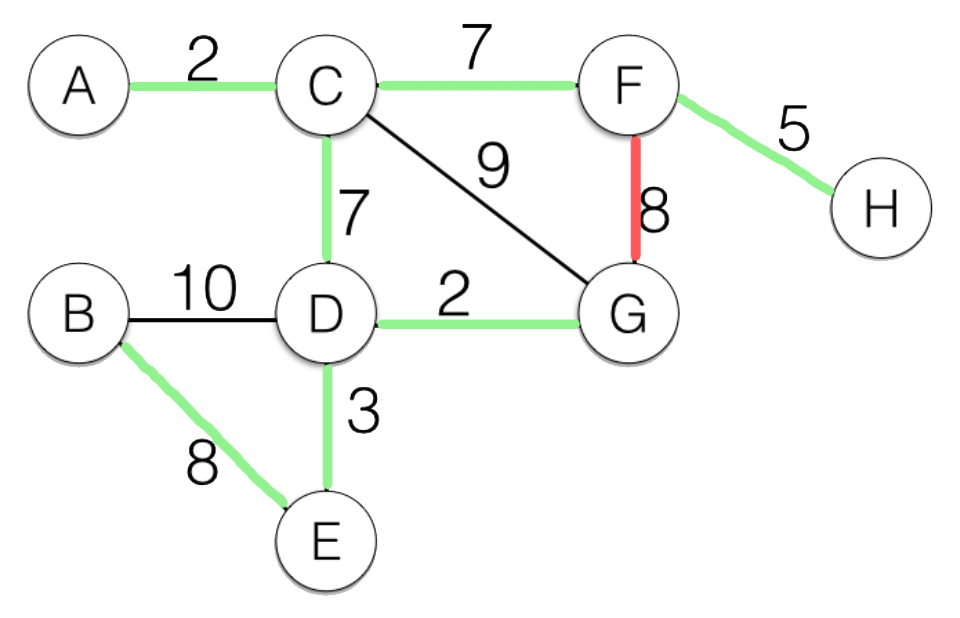
\includegraphics[scale=0.25]{graph8.png}
\newline
(A, C) = 2, OKAY
\newline
(D, G) = 2, OKAY
\newline
(D, E) = 3, OKAY
\newline
(F, H) = 5, OKAY
\newline
(C, D) = 7, OKAY
\newline
(C, F) = 7, OKAY
\newline
(B, E) = 8, OKAY
\newline
(F, G) = 8, REJECTED
\newline
(C, G) = 9
\newline
(B, D) = 10

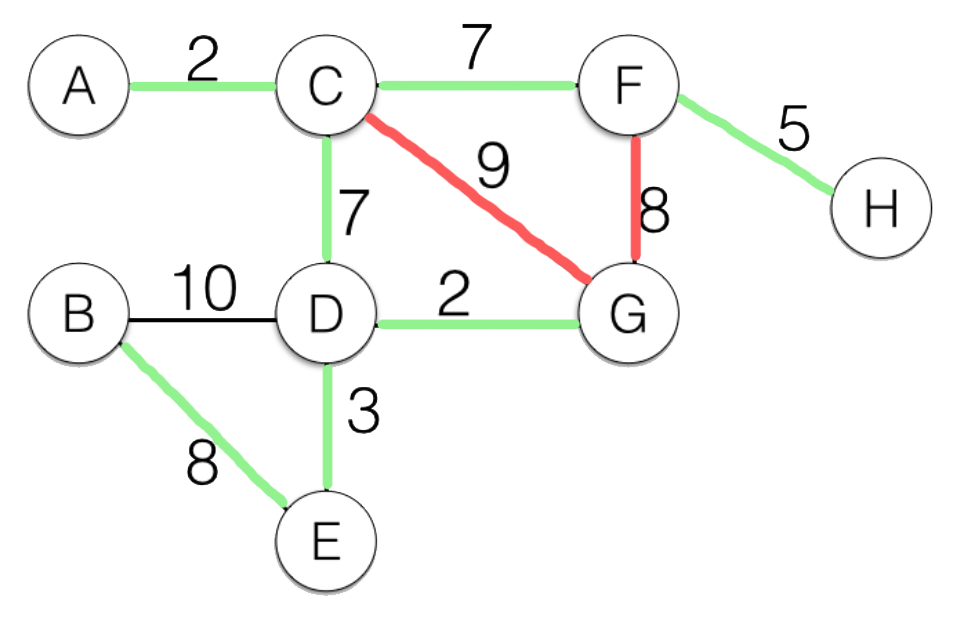
\includegraphics[scale=0.25]{graph9.png}
\newline
(A, C) = 2, OKAY
\newline
(D, G) = 2, OKAY
\newline
(D, E) = 3, OKAY
\newline
(F, H) = 5, OKAY
\newline
(C, D) = 7, OKAY
\newline
(C, F) = 7, OKAY
\newline
(B, E) = 8, OKAY
\newline
(F, G) = 8, REJECTED
\newline
(C, G) = 9, REJECTED
\newline
(B, D) = 10

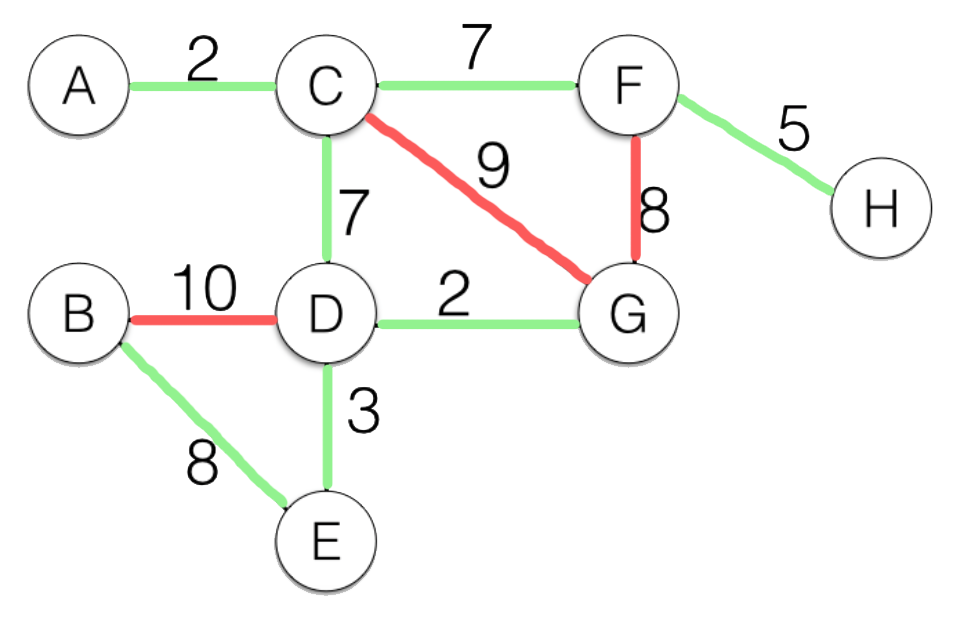
\includegraphics[scale=0.25]{graph10.png}
\newline
(A, C) = 2, OKAY
\newline
(D, G) = 2, OKAY
\newline
(D, E) = 3, OKAY
\newline
(F, H) = 5, OKAY
\newline
(C, D) = 7, OKAY
\newline
(C, F) = 7, OKAY
\newline
(B, E) = 8, OKAY
\newline
(F, G) = 8, REJECTED
\newline
(C, G) = 9, REJECTED
\newline
(B, D) = 10, REJECTED

\subsection{}
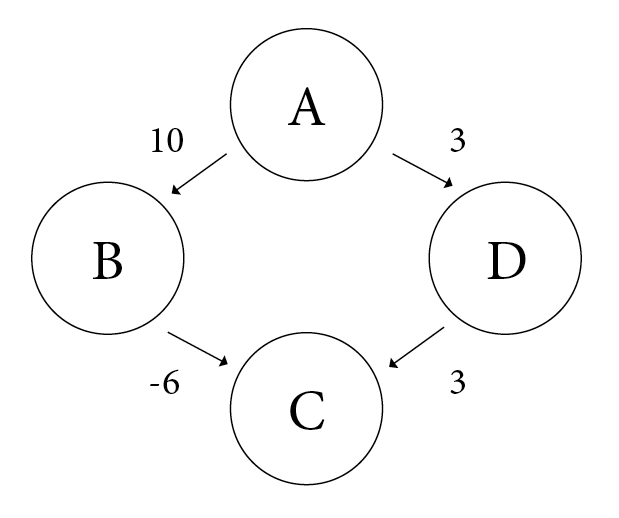
\includegraphics[scale=0.5]{directed-graph.png}
\newline
In moving from A to C:
\newline
d(D) = 3
\newline
d(C) = 6
\newline
Because d(B) = 10 and Dijkstra's algorithm doesn't take negative weight edges into account, it would find ADC as the shortest path, even though ABC has a path length of 4 instead of 6. The ADC path would have lower cost annotations compared to d(B).

\subsection{}
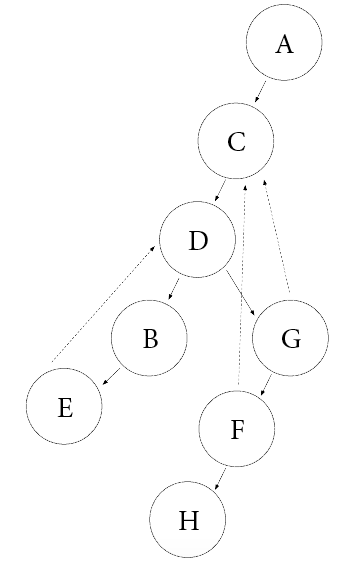
\includegraphics[scale=0.5]{depth-first-spanning-tree.png}
\newline
\begin{table}[h]
\centering
\begin{tabular}{|l|l|l|}
\hline
v & Num(v) & Low(v) \\ \hline
A & 1 & 1 \\ \hline
B & 4 & 3 \\ \hline
C & 2 & 1 \\ \hline
D & 3 & 1 \\ \hline
E & 5 & 3 \\ \hline
F & 7 & 7 \\ \hline
G & 6 & 6 \\ \hline
H & 8 & 7 \\ \hline
\end{tabular}
\end{table}

\end{document}